To further understand how coordination facts work, we present other programs that
take advantage of them.

\subsection{Belief Propagation}

Randomized and approximation algorithms can obtain significant benefits from
coordination directives because although the final program results will not be
exact, they follow important statistical properties and can be computed faster.
An examples of such programs is PageRank~\cite{Lubachevsky:1986:CAA:4904.4801}
and Loopy Belief Propagation~\cite{Gonzalez+al:aistats09paraml}, which is the
focus of this section.

Loopy Belief Propagation (LBP) is an approximate inference algorithm used in
graphical models with cycles~\cite{Murphy99loopybelief}. In its essence, LBP is
a sum-product message passing algorithm where nodes exchange messages with their
immediate neighbors and apply some computations to the messages received.

LBP is an algorithm that maps very well to the graph-based model of LM. The
original algorithm computes the belief of all nodes for several iterations with
synchronization between iterations. However, it is possible to avoid the
synchronization step, if we take advantage of the fact that LBP will converge
even when using an asynchronous approach. So, instead of computing the belief
iteratively, we keep track of all messages sent/received (and overwrite them
when we receive a new one) and recompute the belief asynchronously.
Figure~\ref{fig:coordination:bp} shows the communication patterns for our
application and Fig.~\ref{code:coordination:bp} presents the LM code for the
implementation.

\begin{figure}[h]
   \begin{center}
      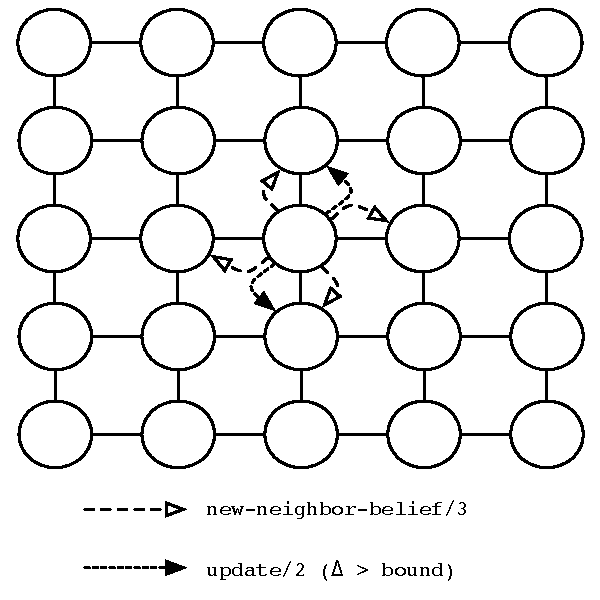
\includegraphics[width=0.3\textwidth]{figures/bp/bp.pdf}
   \end{center}
\caption{LBP: communication patterns}
\label{fig:coordination:bp}
\end{figure}

\begin{figure}[h!]
   \begin{Verbatim}[numbers=left, fontsize=\scriptsize]
neighbor-belief(A, B, Belief),
new-neighbor-belief(A, B, NewBelief)
   -o neighbor-belief(A, B, NewBelief).

check-residual(A, Residual, B),
Residual > bound
   -o update(B).
check-residual(A, _, _) -o 1.

// update belief to be sent to one neighbor
update-messages(A, NewBelief),
!edge(A, B),
neighbor-belief-old(A, B, OldIn),
sent-neighbor-belief(A, B, OldOut),
Cavity = normalize(divide(NewBelief, OldIn)),
Convolved = normalize(convolve(global-potential, Cavity)),
OutMessage = damp(Convolved, OldOut, damping)
   -o Residual = residual(OutMessage, OldOut),
      check-residual(A, Residual, B),
      update-messages(A, NewBelief),
      new-neighbor-belief(B, A, OutMessage),
      sent-neighbor-belief(A, B, OutMessage).

update-messages(A, NewBelief) -o 1.

// if we have two update functions, just run one of them
update(A), update(A) -o update(A).

// make a copy of neighbors beliefs in order to add them up
update(A),
!potential(A, Potential),
belief(A, MyBelief)
   -o [custom addfloats Potential => Belief | B, Belief |
         neighbor-belief(A, B, Belief) |
         neighbor-belief-old(A, B, Belief), neighbor-belief(A, B, Belief) |
         Normalized = normalizestruct(Belief),
         update-messages(A, Normalized), belief(A, Normalized)].
\end{Verbatim}
\caption{LM code for the Loopy Belief Propagation problem.}
\label{code:coordination:bp}
\end{figure}

Belief values are arrays of floats and are represented by \texttt{belief/2}
facts. The first rule (lines 1-3) updates a given neighbor belief whenever a new
belief value is received. This is the highest priority rule since we want to
update the neighbor beliefs before doing anything else. In order to store the
belief values of the neighbor nodes, we use \texttt{neighbor-belief/3} facts,
where the second argument is the neighbor address and the third argument is the
belief value.

The last two rules (lines 26-37) update the belief value of a node. An
\texttt{update/1} fact starts the process. The first rule (lines 27) simply
consumes redundant \texttt{update/1} facts and the second rule (lines 30-37)
performs the belief update by aggregating all the neighbor belief values. The
aggregate in lines 33-37 also derives copies of the neighbors beliefs that need
to be consumed in order to compute the belief value that is going to be sent to
the target neighbor. The aggregate uses a custom accumulator that takes two
arrays and adds the floating point numbers at each index of the array.  The rule
in lines 10-22 iterates through the neighbor belief values and sends new belief
values by performing the appropriate computations on the new belief value of the
current node and on the belief value sent previously.  Once the facts
\texttt{neighbor-belief-old} are fully consumed, the rule in line 24 is fired in
order to consume \texttt{update-messages}.

For each neighbor update, we also check in lines 5-8 if the change in belief
values is greater than \texttt{bound} (a program constant) and then force the
neighbor nodes to update their belief values by deriving \texttt{update(B)}.
This allows neighbor nodes to use updated neighbor values and recompute their
own belief values using better information. The computation of belief values
will then start to converge to their true belief values, independently of the
node scheduling used. However, if we prioritize nodes that receive new neighbor
belief values with a larger \texttt{Residual} then we will converge faster.
Figure~\ref{code:coordination:improved_bp} shows the fourth rule modified with
\texttt{add-priority} in order to increase to priority of neighbor nodes when
the source node has large changes in its belief value.

\begin{figure}[h!]
\begin{Verbatim}[numbers=left,commandchars=\\\{\},fontsize=\scriptsize]
// update belief to be sent to one neighbor
update-messages(A, NewBelief),
!edge(A, B),
neighbor-belief-old(A, B, OldIn),
sent-neighbor-belief(A, B, OldOut),
Cavity = normalize(divide(NewBelief, OldIn)),
Convolved = normalize(convolve(global-potential, Cavity)),
OutMessage = damp(Convolved, OldOut, damping)
   -o Residual = residual(OutMessage, OldOut),
      \underline{add-priority(B, Residual)},
      check-residual(A, Residual, B),
      update-messages(A, NewBelief),
      new-neighbor-belief(B, A, OutMessage),
      sent-neighbor-belief(A, B, OutMessage).
\end{Verbatim}
\caption{Updating the BP program to use priorities.}
\label{code:coordination:improved_bp}
\end{figure}

\subsection{N Queens}

The N-Queens puzzle is the problem of placing N chess queens on an NxN
chessboard so that no pair of two queens attack each
other~\cite{8queens}. The specific challenge of finding all the
distinct solutions to this problem is a good benchmark in designing
parallel algorithms.  Our solution is presented next in
Fig.~\ref{coordination:code:nqueens}.

In our implementation, nodes are the squares of the chessboard. Each
square can communicate with other 4 squares: the adjacent right and
the adjacent left on the same row, and the first non-diagonal square
to the right and to the left on the row below. To represent a
partial/valid board state, we use a list of integers, where each pair
of integers represents a coordinate in which a queen is placed. For
example $[1, 2, 0, 0]$ means that a queen is placed in square $(0, 0)$
and another in square $(1, 2)$. At any given time, many partial states
can be using the same squares. Each square can also have many states
at the same time.

\begin{figure}[ht]
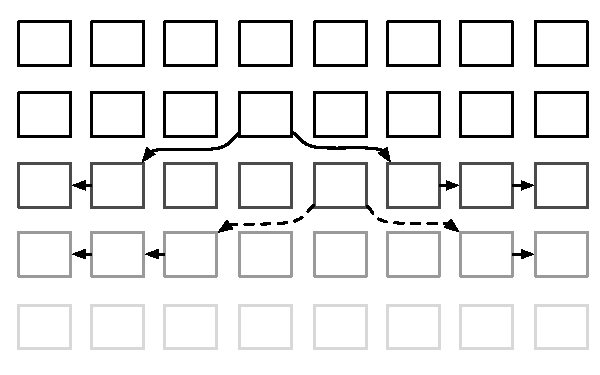
\includegraphics[width=0.4\textwidth]{figures/coordination/nqueens.pdf}
\caption{Concurrent propagation of N-Queens states.}
\label{coordination:fig:nqueens}
\end{figure}

An empty state is instantiated in the top-left square (line 17) and is
then propagated to all squares in the same row (rule in lines
22-24). Once a square $S$ receives a new state $L$, it checks if $S$ can be
incorporated into $L$. For that, it checks if there is no queen on $S$'s
column (rules in lines 29-35), if there is no queen on $S$'s left
diagonal (rules in lines 37-43) and if there is no queen on $S$'s right
diagonal (rules in lines 45-51).

If there is any conflict, we do not derive anything and for that we use the
language expression \texttt{1} (lines 33, 41 and 49), which corresponds to an
empty rule head. If there are no conflicts, this means that it is possible to
add a queen to the current state (line 31). The fact \texttt{send-down/2} is
used to either complete the computation of a valid state (lines 53-54) or to
propagate the state to the row below (lines 55-57) as shown in
Fig.~\ref{coordination:fig:nqueens}.

Most popular parallel implementations of the N-Queens problem
distribute the search space of the problem by assigning incomplete
boards as tasks to threads. Our approach is unusual because the tasks
are the squares of the board.

\begin{figure}[h!]
\begin{Verbatim}[numbers=left,fontsize=\scriptsize]
type list int state.

type left(node, node).
type right(node, node).
type down-left(node, node).
type down-right(node, node).
type coord(node, int, int).
type linear propagate-left(node, state).
type linear propagate-right(node, state).
type linear test-y(node, int, state, state).
type linear test-diag-left(node, int, int, state, state).
type linear test-diag-right(node, int, int, state, state).
type linear send-down(node, state).
type linear new-state(node, state).
type linear final-state(node, state).

propagate-right(@0, []).

propagate-left(A, State)
  -o {L | !left(A, L), L <> A | propagate-left(L, State)},
     new-state(A, State).
propagate-right(A, State)
  -o {R | !right(A, R), R <> A | propagate-right(R, State)},
     new-state(A, State).

new-state(A, State), !coord(A, X, Y)
  -o test-y(A, Y, State, State).

// check if there is no queen on the same column
test-y(A, Y, [], State), !coord(A, OX, OY)
  -o test-diag-left(A, OX - 1, OY - 1, State, State).
test-y(A, Y, [X, Y1 | RestState], State), Y = Y1
  -o 1. // fail
test-y(A, Y, [X, Y1 | RestState], State), Y <> Y1
  -o test-y(A, Y, RestState, State).

// check if there is no queen on the left diagonal
test-diag-left(A, X, Y, _, State), X < 0 || Y < 0, !coord(A, OX, OY)
  -o test-diag-right(A, OX - 1, OY + 1, State, State).
test-diag-left(A, X, Y, [X1, Y1 | RestState], State), X = X1, Y = Y1
  -o 1. // fail
test-diag-left(A, X, Y, [X1, Y1 | RestState], State), X <> X1 || Y <> Y1
  -o test-diag-left(A, X - 1, Y - 1, RestState, State).

// check if there is no queen on the right diagonal
test-diag-right(A, X, Y, [], State), X < 0 || Y >= size, !coord(A, OX, OY)
  -o send-down(A, [OX, OY | State]). // add new queen
test-diag-right(A, X, Y, [X1, Y1 | RestState], State), X = X1, Y = Y1
  -o 1. // fail
test-diag-right(A, X, Y, [X1, Y1 | RestState], State), X <> X1 || Y <> Y1
  -o test-diag-right(A, X - 1, Y + 1, RestState, State).

send-down(A, State), !coord(A, size - 1, _)
  -o final-state(A, State).
send-down(A, State), !coord(A, CX, _), CX <> size - 1
  -o {B | !down-right(A, B), B <> A | propagate-right(B, State)},
     {B | !down-left(A, B), B <> A | propagate-left(B, State)}.
\end{Verbatim}
  \caption{N-Queens problem solved in LM.}
  \label{coordination:code:nqueens}
\end{figure}


\subsection{Heat Transfer}


